\documentclass[a4paper]{scrreprt}
\usepackage{fancyhdr}
\pagestyle{fancy}
\usepackage[english]{babel}
\usepackage[utf8]{inputenc}
\usepackage{graphicx}
\usepackage{url}
\usepackage{textcomp}
\usepackage{amsmath}
\usepackage{lastpage}
\usepackage{pgf}
\usepackage{wrapfig}
\usepackage{fancyvrb}

% Create header and footer
\headheight 27pt
\pagestyle{fancyplain}
\lhead{\footnotesize{Object-Oriented Design, IV1350}}
\chead{\footnotesize{Seminar 1 Solution}}
\rhead{}
\lfoot{}
\cfoot{\thepage\ (\pageref{LastPage})}
\rfoot{}

% Create title page
\title{Seminar 1}
\subtitle{Object-Oriented Design, IV1350}
\author{Sebastian Heimlén heimlen@kth.se}
%\date{\today} Prints today's date
\date{07/04-2016}

\begin{document}

\maketitle

\tableofcontents %Generates the TOC

\chapter{Introduction}

The first task of this seminar was to create a domain model for a vehicle inspection company with the help of a UML class diagram. The domain model should include the functionality \textit{Inspect Vehicle}. The goal of the domain model is to enhance and clarify the requirements specification and portray the reality in which the system will take place.

The second task was to create a system sequence diagram for the same functionality \textit{Inspect Vehicle}. The system sequence diagram shows the interaction between the system under development and the the actors using it. The goal of the system sequence diagram is to simplify development, since  it shows exactly what tasks the system can be told to do, and how it responds to these tasks.

\chapter{Method}

There are certain steps that one follows to create a domain model, these 5 steps was what I followed to produce my DM.

The first step is to use \textit{noun identification}, which means that you create a class of every noun in the requirements specification, therefore the first thing I did was to underline every noun in the requirements specification and then I made a class of each of them.

The second step is to use a \textit{category list} to help you find even more classes, one thing to note is that these two first steps consist of finding classes that could fit in your system, the point here is to find as many classes as possible, since it is easier to remove classes then to find classes later. I wrote down some categories in Excel and started to fill the category list with things I could think of that had with the system to do, I then made a class of each of the objects in the category list. see figure \ref{fig:category}.

\begin{figure}[h]
  \begin{center}
    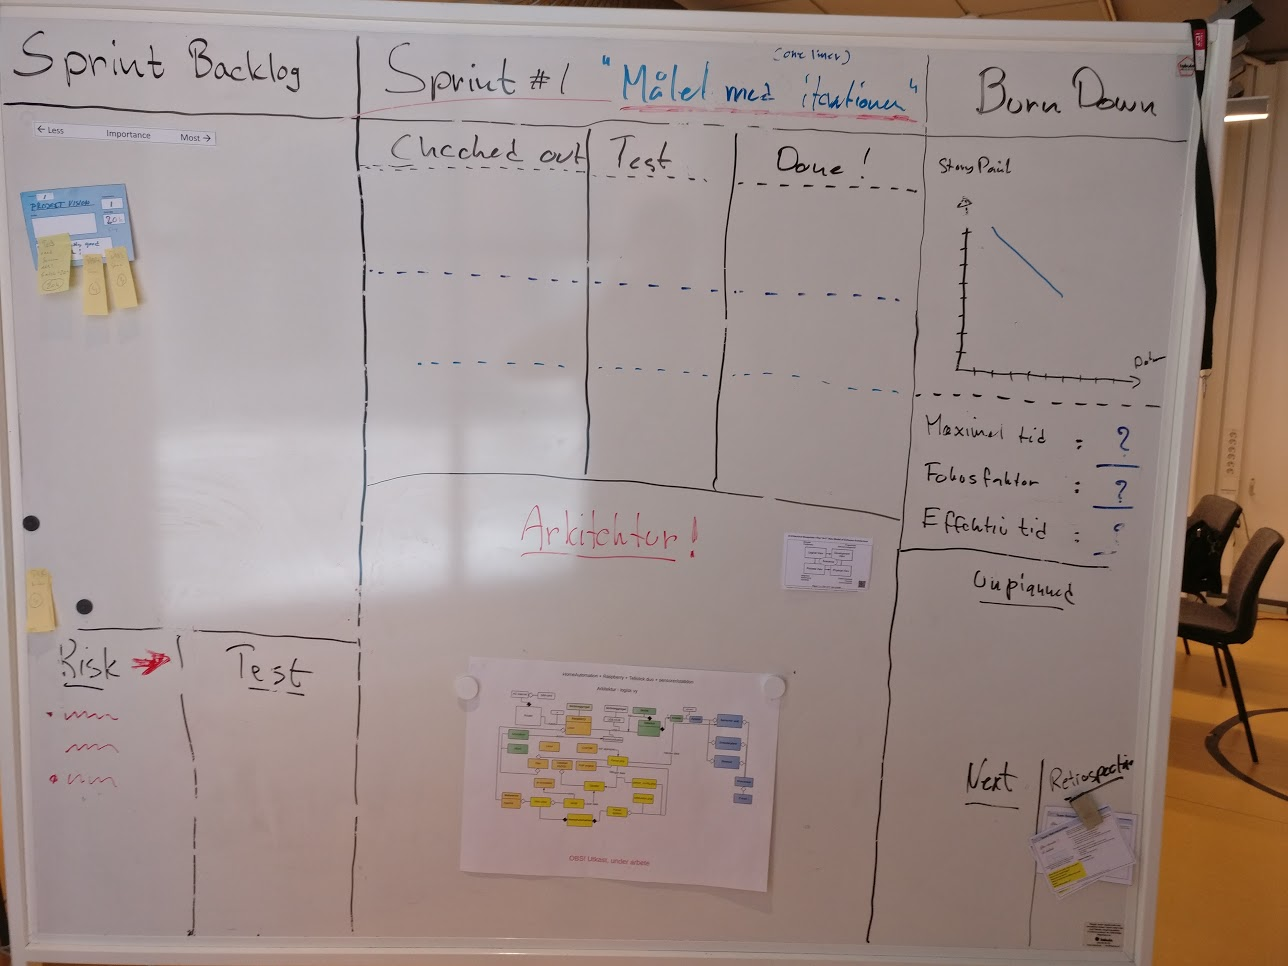
\includegraphics[scale=0.2]{test.jpg}
    \caption{Category list created in Excel}
    \label{fig:category}
  \end{center}
\end{figure}

\noindent In step three you remove classes that are not needed in your specific functionality, here I removed a large part of the classes after re-evaluating the requirement specification and deciding what classes that would be needed to model the specific functionality \textit{inspect vehicle}. For example I removed the class \texttt{ErrorReport} because it had no place in this particular function, \texttt{UpdateVehicleRecord} is another example of a class getting removed because it could lead to a "programmatic DM".

In Step four you consider which classes that should be changed into attributes. An example of a class that I made into an attribute is \texttt{Cost} that instead became an attribute of the class \texttt{PaymentOfInspection}.

The fifth and last step consists of adding associations between classes, the purpose of associations is to clarify the DM and make it easier to see what associations different classes have. When I added my associations I tried to only add the most important associations to avoid cluttering the DM with a lot of associations that did not clarify the model, I based all associations purely on how they associate to each other in \textbf{{reality}} to avoid a "programmatic" DM, I also tried to split the associations evenly between classes to not have a "spider-in-the-web" class, which is a class that has a lot of associations while other parts of the DM has very few associations, since it is preferred to have a DM that is more evenly distributed.\\
\\
While creating a system sequence diagram, which is the second task of the seminar, there is a few things to keep in mind. The first thing that is of importance is to \textbf{only} include events between the actors and the system and the events between the system and external devices such as a display, things like the customer parking his car in the parking lot should not be a part of the SSD. The other thing that is important to note is that the SSD should only include events that is in the required specification of the functionality, if the event is not present in the specification, it should not be added to the SSD.

Creating the SSD was pretty straight forward, I followed each step in the required specification and if it was an event between the actors and the system or/and the system and an external device I added the event to the SSD, this way I got every event in the right order with the right arguments and return values. Lastly I implemented the alternative flows at the right place in the SSD.



\chapter{Result}
\label{sec:result}

These are the results of my work.

First off is the domain model, as mentioned earlier I tried my best to make an even distributed DM, which means that all parts of the DM has an equal amount of associations, I tried to only add the associations that where specified in the requirements as well as the more obvious and important associations between classes, there could be a lot more associations added, but I felt that the current associations suffice and that more would only lead to the DM getting harder to read and understand. see figure \ref{fig:dmodel}.

\begin{figure}[h]
  \begin{center}
    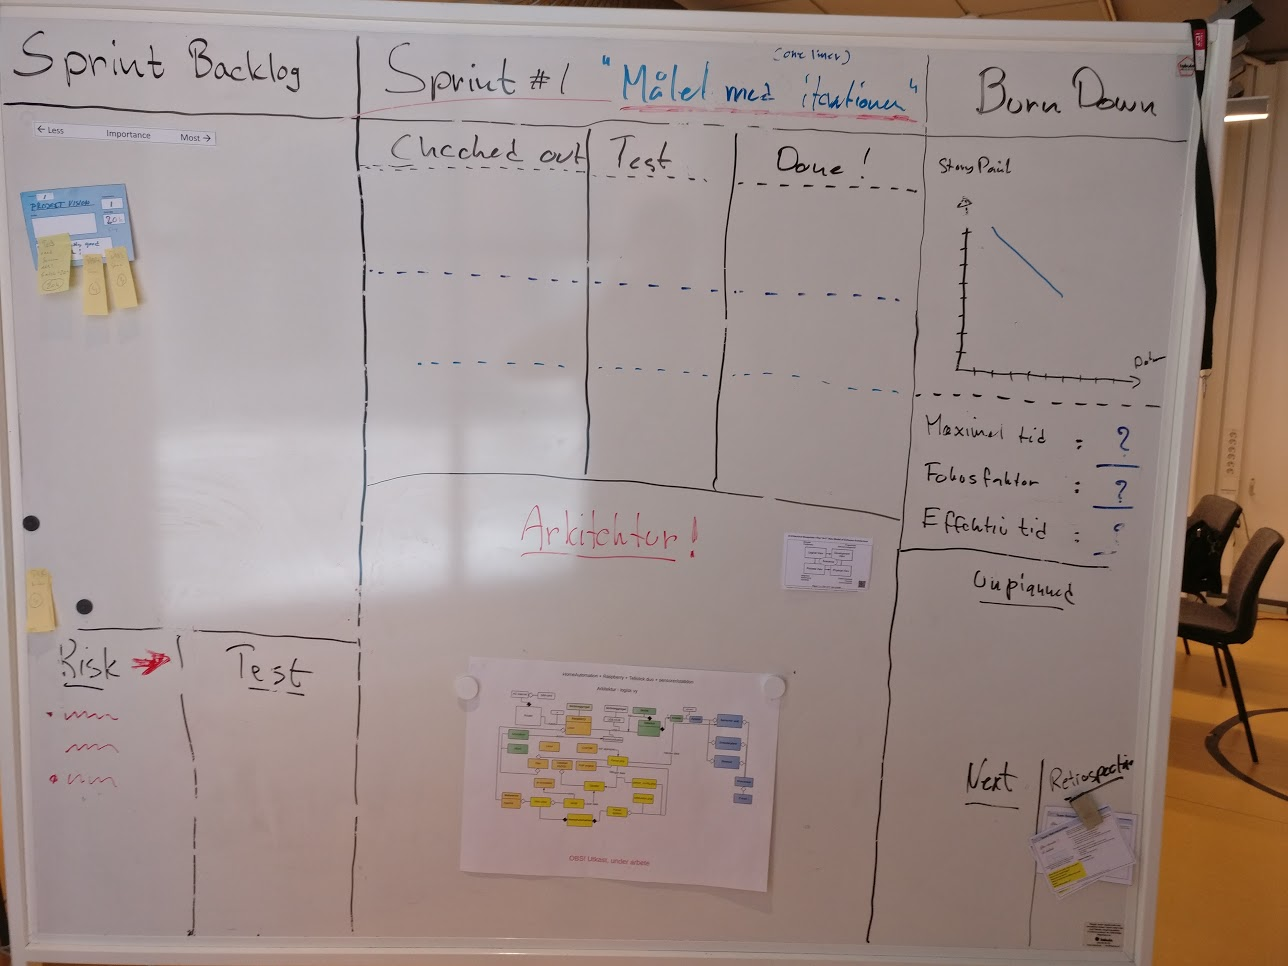
\includegraphics[scale=0.2]{test.jpg}
    \caption{A picture of the created domain model.}
    \label{fig:dmodel}
  \end{center}
\end{figure}

\noindent The system sequence diagram looked straightforward at first, but became slightly more complicated when it was time to implement the alternative flows. This SSD provides an overview of the events between the system and the actors using it. It mostly consists of program calls to different external devices, but there are also some loops that are required to meet the requirements specification, as well as a if-else statement to make sure the customer can pay with both credit card as well as cash. see figure \ref{fig:ssd}.

\begin{figure}[h]
  \begin{center}
    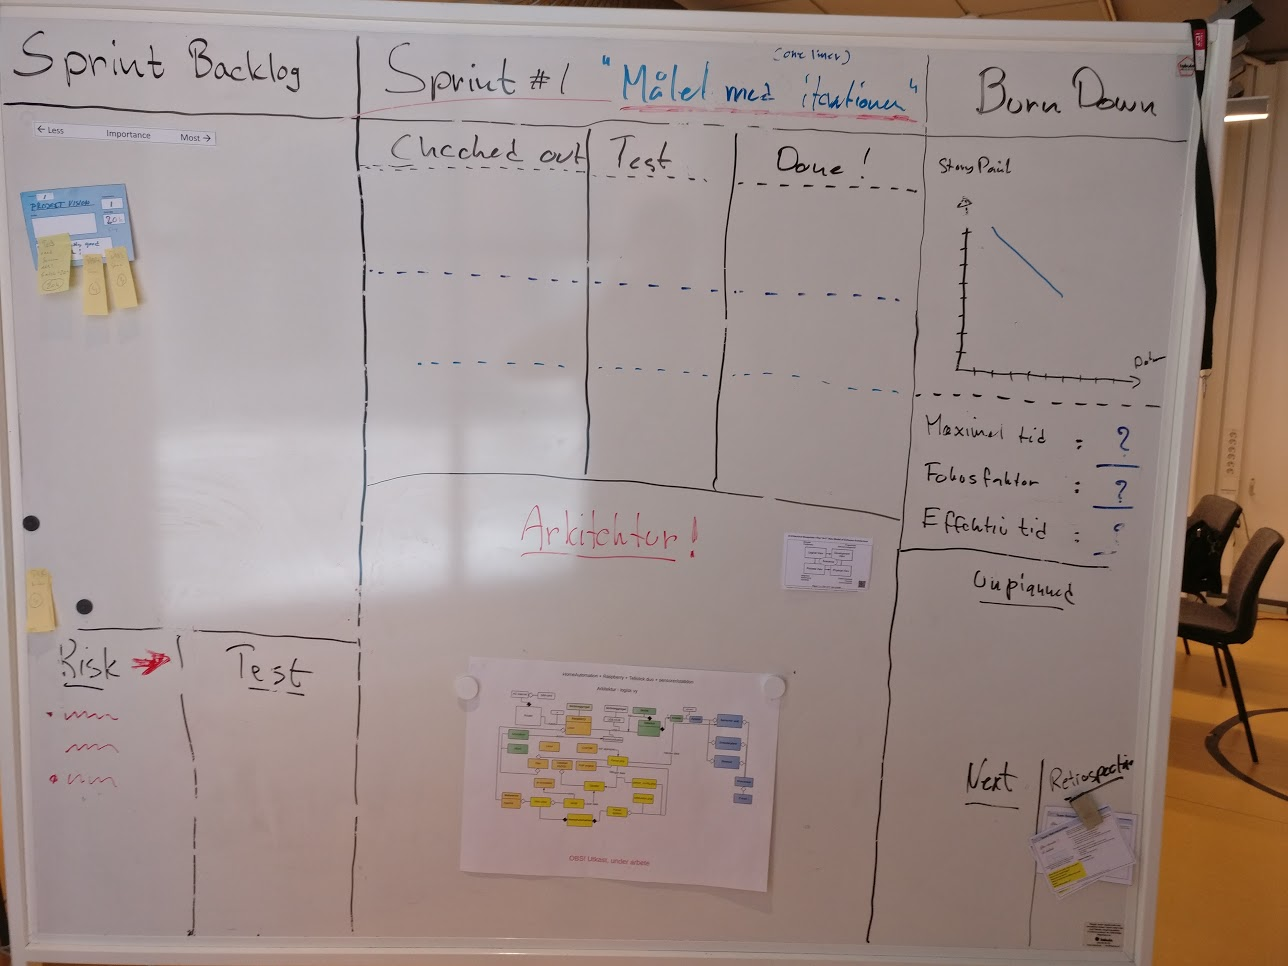
\includegraphics[scale=0.2]{test.jpg}
    \caption{System sequence diagram.}
    \label{fig:ssd}
  \end{center}
\end{figure}

\chapter{Discussion}

I am pleased with both my domain model and my system sequence diagram, my DM has a reasonable amount of classes, it is neither "naïve" or "programmatic" and the associations are distributed in a good manner. The SSD, for all I know and can see, correctly implements the right events in the right order and clearly displays the interactions between the actors, the system and the external devices. however I feel that there are some things that could be added which would make these models even better, things that were unclear in the requirements specification.

First off, me and my friends discussed adding a class called \texttt{Queue} to the domain model that would have an association with \texttt{Queuesystem} and \texttt{Customer} because as the function is presented now, we have customers that have queue numbers, but we do not have a queue, neither do we know how customers acquire a queue number, do they get it when they book the inspection, or do they just "drop-in" and wait in the queue until their queue number is up? Another thing we discussed is how much information about the customer the system needs, for administrative reasons, do the system need the customers name, address, phone number etc. or do the drivers license and the actual car suffice? If the system needs this information, should that then be added as a class in the DM? There are many questions here regarding the requirements specification, we came to the conclusion that these specific questions does not really have to have an answer in the function \textit{Inspect Vehicle}, they do not really matter in this case, but I think that adding some sort of explanation to how the queue number is granted would lower the risk of a misunderstanding between the client and the system developers.

Another \textbf{enormous} flaw with the requirements specification as it is currently stated is that it does not specify what the system should do if the authentication of the payment does not go through for some reason. As the system currently is designed it will carry on with the inspection even if the authentication is declined, which in turn leads to the company not getting paid for the inspection while still performing it, this is of course a completely unacceptable situation and a huge flaw in the requirements specification that leads to a major flaw in the SSD which in turn leads to wrongful development of the system. It is not up to us as developers to take matters in our own hands and correct this issue, however a possible solution would be to abort the transaction and let the customer redo the transaction in case of an authentication error.

\end{document}
